

\section{\TITLE{}: A Proof-Serving System}
\label{sec:design}



We introduce \TITLE{}, a distributed proof-serving system for cloud-hosted zkML inference. \TITLE{} targets workloads for which monolithic proof generation incurs prohibitive latency or exceeds the memory capacity of a single machine. The system partitions each zkML inference request into fine-grained proving jobs and distributes their execution across a pool of prover workers. \TITLE{} coordinates job inputs, reusable proving artifacts, per-job runtime and memory profiles, and resource-aware scheduling, while relying on an underlying zkML backend to generate each proof.






\definecolor{controlFill}{HTML}{EAF2FF}
\definecolor{execFill}{HTML}{EAF7F2}
\definecolor{storeFill}{HTML}{FFF3E0}
\definecolor{neutralFill}{HTML}{F8FAFC}
\definecolor{borderColor}{HTML}{4A5568}
\definecolor{textMuted}{HTML}{64748B}

\begin{figure}[t]
\centering
\begin{tikzpicture}[
font=\fontsize{9.3pt}{10.5pt}\selectfont,
component/.style={
draw=borderColor,
rounded corners=2pt,
line width=0.6pt,
align=center,
inner sep=6.2pt,
fill=neutralFill
},
controlbox/.style={
component,
fill=controlFill
},
execbox/.style={
component,
fill=execFill
},
storebox/.style={
component,
fill=storeFill
},
smallbox/.style={
component,
fill=white,
inner sep=5.2pt
},
ctrl/.style={
-{Latex[length=2mm]},
line width=0.75pt,
draw=black!75
},
ctrlbi/.style={
{Latex[length=2mm]}-{Latex[length=2mm]},
line width=0.75pt,
draw=black!75
},
data/.style={
-{Latex[length=2mm]},
line width=0.75pt,
dashed,
draw=black!65
},
lab/.style={
font=\small,
align=center,
fill=white,
inner sep=1.5pt,
text=black!80
}
]

% Main components
\node[component, minimum width=2.05cm, minimum height=0.68cm]
(client) at (0,0) {Client};

\node[controlbox, minimum width=3.75cm, minimum height=0.95cm, below=0.98cm of client]
(orch) {\textbf{Orchestrator}};

\node[execbox, minimum width=6.15cm, minimum height=2.72cm, below=1.18cm of orch]
(exec) {};

\node[
anchor=north west,
font=\fontsize{9.3pt}{10.5pt}\selectfont\bfseries,
text=black!85,
align=left
]
at ([xshift=0.18cm,yshift=-0.14cm]exec.north west)
{Prover execution\\layer};

\node[
anchor=north east,
font=\small,
text=textMuted
]
at ([xshift=-0.18cm,yshift=-0.20cm]exec.north east)
{worker machine(s)};

\node[smallbox, minimum width=2.85cm, minimum height=0.62cm]
(manager) at ([yshift=0.42cm]exec.center)
{Worker manager};

\node[smallbox, minimum width=1.72cm, minimum height=0.66cm]
(pw1) at ([xshift=-1.16cm,yshift=-0.62cm]exec.center)
{Prover\\worker};

\node[smallbox, minimum width=1.72cm, minimum height=0.66cm]
(pw2) at ([xshift=1.16cm,yshift=-0.62cm]exec.center)
{Prover\\worker};

\node[storebox, minimum width=4.75cm, minimum height=0.9cm, below=1.10cm of exec]
(store) {\textbf{Artifact store}};

% Client request / response paths
\draw[ctrl] ([xshift=-0.48cm]client.south) --
node[lab, left] {request}
([xshift=-0.48cm]orch.north);

\draw[ctrl] ([xshift=0.48cm]orch.north) --
node[lab, right] {output +\\proofs}
([xshift=0.48cm]client.south);

% Orchestrator / worker-manager control path
\draw[ctrlbi] (orch.south) --
node[lab, right] {jobs / status / refs}
(manager.north);

% Local dispatch
\draw[ctrl] ([xshift=-0.42cm]manager.south) -- (pw1.north);
\draw[ctrl] ([xshift=0.42cm]manager.south) -- (pw2.north);

% Storage paths
\draw[data] (orch.east) -- ++(1.08,0) |-
node[pos=0.72, lab, right] {large job\\objects}
(store.east);

\draw[data] (exec.south) --
node[lab, right] {data / proofs\\artifacts}
(store.north);

% Legend
\node[font=\small, below=0.34cm of store] {
\tikz{\draw[ctrl] (0,0) -- (0.5,0);} control/RPC
\quad
\tikz{\draw[data] (0,0) -- (0.5,0);} storage/data
};

\end{tikzpicture}
\caption{
Architecture of \TITLE{}. The orchestrator creates and schedules proving jobs across worker machines, while an artifact store holds large job inputs, proofs, and reusable setup artifacts.
}
\label{fig:architecture}
\end{figure}

\subsection{System Overview}
\label{sec:system-overview}

Figure~\ref{fig:architecture} shows the architecture of \TITLE{}. The system separates request coordination from proof execution across three components: an orchestrator, worker machines that run prover processes, and a shared artifact store.

\noindent\textbf{Orchestrator.}
The orchestrator partitions each inference graph into proving jobs, tracks their execution and proof-composition relationships, and dispatches them to workers. Each job is assigned a stable content hash derived from its partition and circuit-defining settings, which indexes historical runtime and memory profiles as well as cached proving artifacts. These profiles guide scheduling, while completed proof and output references are recorded until all jobs for the request finish.

\noindent\textbf{Prover execution layer.}
Each worker machine runs a worker manager and a pool of prover workers. The manager reports local capacity and requests work from the orchestrator, which assigns jobs using the scheduling policy in Section~\ref{sec:resource-aware-scheduling}. Prover workers load job inputs, reuse or generate setup artifacts as needed, invoke the configured zkML backend, and store resulting proofs and outputs in the shared artifact store. They also report runtime and memory measurements used to refine future job profiles.

\noindent\textbf{Artifact store.}
The artifact store holds request-specific data, including model inputs, intermediate tensors, outputs, and proofs, allowing workers to access large objects directly while the orchestrator exchanges lightweight references. It also caches reusable compiled representations and proving keys under each job's content hash. Cache usage is bounded by a configurable storage budget, with eviction based on recency and regeneration cost. The interface supports both shared filesystems and remote object storage; our cloud deployment uses AWS S3~\cite{aws-s3}.




% \begin{figure}[t]
%     \centering
%     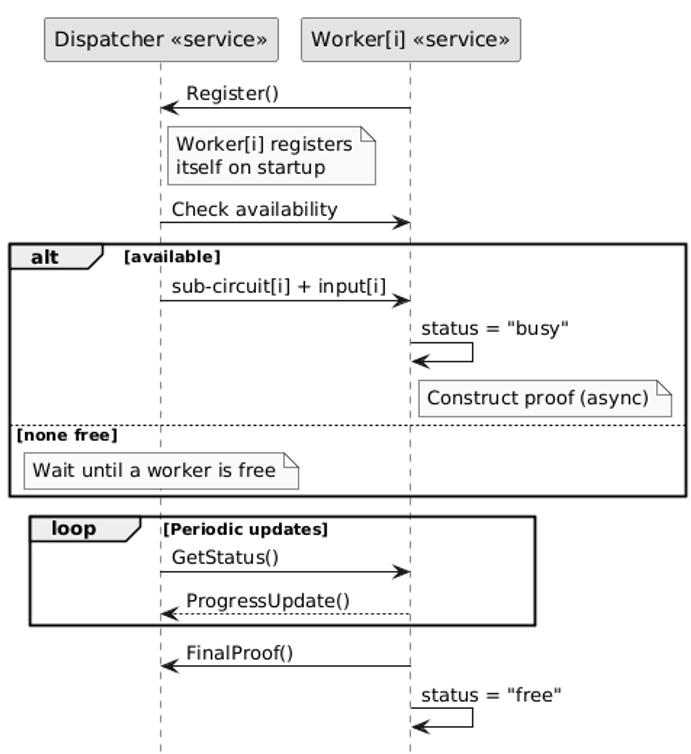
\includegraphics[width=0.9\linewidth]{figures/arch2.png}
%     \caption{Architecture and workflow of \TITLE{}}
%     \label{fig:architecture}
% \end{figure}

% \noindent\textbf{Model Splitting.}
% In practice, extracting a submodel requires preserving the ONNX tensor names and metadata that define its interface. \TITLE{} derives each partition's inputs and outputs from the graph dataflow, extracts the corresponding ONNX submodel, and preserves the original tensor names at the partition boundary. These names are later used to bind materialized tensor values to the correct submodel inputs.

% Although \TITLE{} relies on standard ONNX extraction mechanisms, producing usable proving jobs requires care. Modern ONNX models are not simple operator chains: tensors may be reused across branches, merged by later operators, or produced by shape and bookkeeping nodes. \TITLE{} therefore derives each partition interface from the graph dataflow, preserving the original tensor names, shapes, types, constants, and initializers needed to execute the extracted submodel independently. This ensures that even models with branching structure, such as residual blocks, can be decomposed into submodels whose inputs can later be bound to materialized runtime tensor values.

% \noindent\textbf{Profiling.}
% The profiling interface is backend-agnostic. Workers report execution stages and resource measurements through a common abstraction, and the orchestrator stores them in the corresponding cost profile. Backends with coarse instrumentation can report coarse stages, while backends with richer instrumentation can expose finer-grained proving stages or additional resource metrics. This allows \TITLE{} to use more detailed backend information when available without changing the scheduler's core placement policy.

\subsection{Self-Contained Proving Jobs}
\label{sec:self-contained-proving-jobs}

Partitioning determines the computation assigned to each proving job, but not the request-specific boundary tensors needed to construct its witness. If these values were produced only when upstream jobs completed, proving would inherit execution dependencies between partitions. \TITLE{} avoids this by materializing all partition-boundary tensors before distributed proving begins.

For each request, the orchestrator augments the ONNX graph to expose boundary tensors as additional outputs, executes the graph once, and records the resulting values by their ONNX names. Because extracted partitions preserve these names at their interfaces, each job can be supplied with the inputs required for witness generation before it is scheduled. Jobs are therefore self-contained and can execute independently, subject only to worker availability and resource constraints.

The additional ONNX execution only supplies witness inputs; it does not establish correctness. Each partition is verified by its own proof, and the composition procedure in Section~\ref{sec:proof-composition} checks consistency across partition boundaries so that the job-level proofs together represent one valid end-to-end inference.

\subsection{Resource-Aware Job Scheduling}
\label{sec:resource-aware-scheduling}

\TITLE{} supports concurrent client requests, each of which expands into a set of independently executable proving jobs. A request-oblivious scheduler could place all jobs in a single global queue and assign them in arrival order. However, optimizing the completion of individual jobs does not necessarily optimize request completion. A request finishes only after all of its proving jobs have completed and the resulting proofs are available. Interleaving jobs from many requests may therefore leave several requests partially complete. Job placement must also account for memory demand, since an available worker slot does not imply that the host has sufficient memory to execute another proving job. \TITLE{} addresses these considerations with a request-aware scheduling policy that combines FIFO-biased fair sharing across requests, longest-estimated-runtime-first ordering within each request, and host-level admission control that limits execution according to estimated memory demand.

\subsubsection{Resource Profiles and Memory-Aware Admission}

\TITLE{} maintains a resource profile for each proving job, indexed by its stable content hash, that records expected runtime and peak memory demand. Runtime estimates are used to prioritize jobs within a request, while memory estimates determine whether additional work can be admitted on a worker machine. Profiles persist across requests and are refined using measurements from completed executions. When no prior measurement is available, \TITLE{} initializes the profile using backend-provided information such as EZKL's circuit-sizing metadata.

Admission considers both worker availability and memory capacity. Let \(A_h\) denote the jobs currently executing on worker machine \(h\), \(M(h)\) its memory budget, and \(P(j)\) the estimated peak memory of job \(j\). A pending job \(q\) is admitted only if

\[
    \sum_{j \in A_h} P(j) + P(q) \leq M(h).
\]

\TITLE{} reserves each active job's estimated peak memory for its full execution. In the steady-state serving path, reusable setup artifacts are typically already available, and the largest online memory demand occurs during proof generation. We therefore use a single whole-job peak estimate rather than phase-specific reservations, keeping admission conservative and simple.


\subsubsection{\textbf{Scheduling Policy}}

Algorithm~\ref{alg:cost-aware-scheduling} shows how the orchestrator selects a proving job when a worker machine requests additional work. \TITLE{} maintains pending requests in arrival order and scans the queue from the front. For each request, the scheduler considers its pending jobs in decreasing order of estimated runtime and assigns the first job that satisfies the memory-admission rule on the requesting machine. After assigning a job, the request moves to the back of the queue if it still has pending work. This FIFO-biased fair-sharing policy gives older requests the first scheduling opportunity while preventing a request with many jobs from continuously occupying the worker pool. If none of a request's jobs fits within the machine's remaining memory budget, the scheduler skips that request and continues scanning the queue. Prioritizing longer-running jobs within each request allows expensive work to begin earlier, reducing the likelihood that one long job remains after the request's shorter jobs have completed.


% Whenever a worker machine requests additional work, the orchestrator first chooses a pending request and then selects a job from that request.
% At the request level, \TITLE{} maintains a queue of pending requests in arrival order. When a worker machine requests work, the scheduler scans the queue from the front and selects the first request containing a job that fits within the machine's remaining memory budget. After assigning one job, the request is moved to the back of the queue if it still has pending work. This gives older requests the first scheduling opportunity while allowing other requests to make progress before the same request is considered again. If none of a request's jobs fits on the requesting machine, the scheduler skips that request and continues scanning the queue.
% Within the selected request, jobs are considered in decreasing order of estimated runtime. Since a request completes only after all of its jobs finish, starting longer-running jobs earlier reduces the likelihood that one remains after the shorter jobs have completed.

\subsubsection{\textbf{Worker Pool Management}}

Each worker machine runs a worker manager that maintains a local pool of prover workers. Rather than pushing jobs to machines, the orchestrator waits for worker managers to request work. When an idle prover worker is available, or another worker can be started without exceeding the machine's configured worker limit, the worker manager requests a job from the orchestrator. The request includes the machine's current state, including its active jobs and available worker slots, so that the orchestrator can determine which pending jobs are suitable for that machine. The orchestrator applies Algorithm~\ref{alg:cost-aware-scheduling} and returns at most one job that satisfies the scheduling and memory-admission rules. If no suitable job is available, it returns no assignment and the worker manager retries later.

After receiving a job, the worker manager dispatches it to an idle prover worker or starts a new worker when needed. Prover workers that remain idle for a configurable timeout are shut down. This pull-based design allows scheduling decisions to use machine state reported at assignment time, while separating global job selection at the orchestrator from local worker management on each machine.


% \subsubsection{Worker Pool Management}

% \TITLE{} uses a pull-based worker model to apply the scheduling policy across multi-worker hosts. When local capacity becomes available, each worker manager requests additional work from the orchestrator and includes the host's current execution state. The orchestrator applies Algorithm~\ref{alg:cost-aware-scheduling} using this reported state. If no pending job satisfies the scheduling and memory-admission rules for the host, the orchestrator returns no assignment for that scheduling attempt.

% When a job is assigned, the worker manager dispatches it to an idle prover worker when one is available. If no worker is idle and the host has not reached its configured worker limit, the manager starts another worker process and assigns the job to it. Worker processes that remain idle for a configurable timeout are shut down. This allows the number of prover workers on each host to grow and shrink with available work, while request ordering and memory-admission decisions remain at the orchestrator.

\begin{algorithm}[t]
\caption{Selecting a proving job for worker machine \(h\)}
\label{alg:cost-aware-scheduling}
\begin{algorithmic}[1]
\State \(C \gets \sum_{j \in A_h} P(j)\)
\For{each pending request \(r\) in FIFO-biased fair-share order}
    \For{each pending job \(q\) in \(r\), ordered by decreasing estimated runtime}
        \If{\(C + P(q) \leq M(h)\)}
            \State assign \(q\) to worker machine \(h\)
            \State \textbf{return}
        \EndIf
    \EndFor
\EndFor
\State return no assignment
\end{algorithmic}
\end{algorithm}


% \subsection{Resource-Aware Job Scheduling}
% \label{sec:resource-aware-scheduling}
% \TITLE{} supports concurrent client requests, each of which is split into a dependency graph of proving jobs. A naive scheduler could place all runnable jobs into a single global queue and assign them to workers in arrival order. However, maximizing \textit{job} throughput does not necessarily minimize \textit{request} latency. A request completes only after \textit{all} of its jobs finish and their proofs are assembled. As a result, aggressively interleaving jobs from many requests can leave many requests partially complete, inflating end-to-end latency and tail completion time. To reduce request-level latency, \TITLE{} uses a request-aware scheduling policy that accounts for  memory limits, fairness, and straggling jobs. 

% % \vspace{0.3em}
% \subsubsection{\textbf{Job Cost Profiles}}

% To make scheduling decisions before a job runs, \TITLE{} needs an estimate of how expensive that job will be. The scheduler therefore maintains a cost profile for each proving job. A cost profile summarizes the job's expected runtime and memory demand, including the peak memory expected during each execution phase. \TITLE{} tracks these metrics across common phases such as setup, input loading, circuit compilation, witness generation, and proof generation, while allowing proving backends to expose additional backend-specific phases when available.

% The profiles themselves are keyed by the content hash of the ONNX submodel used to construct the proving job. This works well for \TITLE{} because the same submodels are often reused across many requests, so their observed runtime and memory behavior can be reused. The key can be extended in deployments where backend, host, or configuration choices affect proving cost. When no matching profile exists, \TITLE{} initializes one from static features available at compilation time, such as circuit size, operator mix, and submodel size. These initial estimates are conservative to avoid admitting more work than a host can safely run. After a job completes, the worker reports observed runtime and per-phase peak memory usage, which \TITLE{} uses to refine the profile for future requests. The scheduler uses the resulting profiles in two places. Estimated execution time is used to order runnable jobs within a request, while phase-level memory estimates are used for host-level admission control.

% \subsubsection{\textbf{Memory-Aware Admission Control}}

% Before assigning a job to a worker, \TITLE{} checks whether the target host has enough usable memory to safely admit the job. Here, a host is a physical or virtual machine that may run multiple worker processes. Since those workers share memory, worker availability alone is not a safe placement signal. To account for this, each host runs a lightweight agent that maintains a local view of execution state. Workers report job status and phase transitions to the agent, which reports active jobs, current phases, and usable memory to the orchestrator.

% Using this reported state, the orchestrator applies a memory admission rule. Let \(A_h\) be the set of active jobs on host \(h\), and let \(M(h)\) be the usable memory budget of \(h\). For each active job \(j\), the scheduler reserves memory for the largest phase that the job may still execute, including its current phase. We denote this remaining peak-memory estimate by \(R(j)\). For a queued job \(q\), which has not started yet, the scheduler reserves memory for the largest phase in the entire job and denotes this estimate by \(P(q)\). The scheduler admits \(q\) on \(h\) only if
% \[
%     \sum_{j \in A_h} R(j) + P(q) \leq M(h).
% \]


% This admission rule protects against future memory peaks, not just current usage. A running job may be in a low-memory phase now but still enter a higher-memory phase later. At the same time, the rule does not reserve a job's original peak forever. Once a job passes a high-memory phase, its remaining peak can decrease. This allows the scheduler to recover memory capacity as jobs progress and to admit additional work before all currently running jobs have finished.


% \begin{algorithm}[t]
% \caption{Cost-aware proving job selection for host $h$}
% \label{alg:cost-aware-scheduling}
% \begin{algorithmic}[1]
% \State $C \gets \sum_{j \in A_h} R(j)$
% \For{each request $r$ in FIFO-biased fair-share order}
%     \For{each runnable job $q$ in $r$, ordered by decreasing estimated execution time}
%         \If{$C + P(q) \leq M(h)$}
%             \State assign $q$ to host $h$
%             \State \textbf{return}
%         \EndIf
%     \EndFor
% \EndFor
% \State no job is assigned to $h$
% \end{algorithmic}
% \end{algorithm}


% \subsubsection{\textbf{Scheduling Policy}}

% Algorithm~\ref{alg:cost-aware-scheduling} shows how the orchestrator selects work when a host requests a job. The scheduler scans pending requests in FIFO-biased fair-share order. Fair sharing prevents a large request with many submodel jobs from monopolizing the worker pool, while FIFO bias gives older requests priority and improves request-level latency. FIFO order is not enforced strictly: requests whose runnable jobs are temporarily infeasible on the target host are skipped for the current scheduling attempt, preventing head-of-line blocking.

% Within each request, runnable jobs are considered in decreasing order of estimated execution time and are admitted only if they satisfy the host-level memory admission rule. This longest-processing-time-first policy reduces straggler effects because a request cannot complete until all of its proving jobs have finished. Together, these choices let the scheduler prioritize fairness across requests, reduce request tail latency within each request, and avoid unsafe host placements without introducing head-of-line blocking.

% \subsubsection{\textbf{Worker Pool Management}}
% \TITLE{} uses a pull-based worker model to apply the scheduling policy on multi-worker hosts. Each host agent periodically requests work from the orchestrator and includes the current host state in the request. The orchestrator applies Algorithm~\ref{alg:cost-aware-scheduling} using this reported state. If no queued job satisfies the scheduling and memory-admission rules for that host, the orchestrator returns no assignment for that scheduling attempt. When the orchestrator assigns a job, the host agent dispatches it to an idle worker if one is available. If no worker is idle and the host has not reached its worker limit, the agent starts a new worker process and assigns the job to it. Workers that remain idle for a configurable timeout are shut down. This keeps the worker pool elastic while leaving request ordering, straggler handling, and memory admission centralized at the orchestrator.


\begin{table*}[t]
\centering
\small
\setlength{\tabcolsep}{5pt}
\renewcommand{\arraystretch}{1.15}
\begin{tabular}{l c c c r c l}
\toprule
\textbf{Model} &
\textbf{Input} &
\textbf{\# Params} &
\textbf{Quant.} &
\textbf{\# ZK Constraints} &
\textbf{\# Submodels} &
\textbf{Dominant Ops} \\
\midrule

MobileNetV2
  & $3 \times 224 \times 224$
  & 3.5M
  & INT8
  & 67,108,864
  & 98
  & Conv./Depthwise Conv. \\

MNIST-GAN Gen.
  & 100-dim.\ latent
  & 0.53M
  & INT8
  & 8,928,903
  & 12
  & Dense/Transposed Conv. \\

NanoGPT (4L)
  & Seq.\ len.\ 64
  & 4.2M
  & INT16
  & 16,777,216
  & 192
  & Attention/MLP \\

NanoGPT (10L)
  & Seq.\ len.\ 64
  & 10.5M
  & INT16
  & 49,361,603
  & 487
  & Attention/MLP \\

TinyBERT
  & Seq.\ len.\ 96
  & 14.5M
  & INT8
  & 8,388,608
  & 120
  & Attention/MLP \\

\bottomrule
\end{tabular}
\caption{
Models used in the evaluation. For each model, we report the input size, parameter count, quantization precision, number of ZK constraints, number of submodels produced by \TITLE{}, and dominant operation classes.
}
\label{tab:models}
\end{table*}


% \subsection{Fault Tolerance and Job Recovery}
% \label{sec:fault-tolerance}

% \TITLE{} recovers from prover-worker and worker-machine failures at job granularity. Because jobs execute independently and completed outputs are stored in the shared artifact store, failures do not require an entire request to restart. Interrupted jobs are returned to the scheduling queue and retried, while completed jobs remain available for the final response.

% The orchestrator tracks each job as \textsc{Ready}, \textsc{Running}, \textsc{Done}, or \textsc{Failed}. Workers periodically report progress, and a running job whose worker fails or stops reporting is returned to \textsc{Ready} for reassignment. Jobs that exceed their retry limit become \textsc{Failed} and terminate the request.

% Request and job metadata are persisted so that execution can also resume after an orchestrator restart. Completed jobs remain valid, while interrupted or lost assignments are rescheduled. Thus, failures may delay a request, but completed proof work is preserved and only unfinished jobs must be repeated.

\subsection{Composing Partitioned Proofs}
\label{sec:proof-composition}

Valid job-level proofs do not by themselves establish a valid execution of the full model, because adjacent jobs could use different values at a shared boundary. For partitions \(P_i\) and \(P_j\), where \(P_i\) outputs \(y_i\) and \(P_j\) consumes \(x_j\), the proofs correspond to the same execution only if \(x_j = y_i\).

\TITLE{} enforces this equality using the commitment-swapping approach from prior work on split proofs~\cite{ezkl-splitting}. Each proof commits to its boundary inputs and outputs without revealing them. For boundary \(P_i \rightarrow P_j\), \TITLE{} verifies \(P_j\)'s proof using the commitment to \(P_i\)'s output in place of the commitment to \(P_j\)'s input. If the underlying values differ, verification fails. Applying this check at every boundary ensures that the job-level proofs represent one consistent execution while keeping intermediate tensors private.

